\documentclass[xcolor=pdflatex,dvipsnames,table]{beamer}
\usepackage{epsfig,graphicx}
\usepackage{palatino}
\usepackage{fancybox}
\usepackage{relsize}
\usepackage[procnames]{listings}
\usepackage{hyperref}
\usepackage{qtree} % needed?
\usepackage{booktabs}
\usepackage{dirtree}
\usepackage[normalem]{ulem}


% fatter TT font
\renewcommand*\ttdefault{txtt}
% another TT, suggested by Alex
% \usepackage{inconsolata}
% \usepackage[T1]{fontenc} % needed as well?


\newcommand{\scale}{0.7}

\newcommand{\todo}[1]{{\emph{TODO: #1}}}
\newcommand{\martin}[1]{{\color{blue} Martin: #1}}
\newcommand{\abcdef}[1]{{\color{red} Author2: #1}}

% uncomment following for final submission
%\renewcommand{\todo}[1]{}
%\renewcommand{\martin}[1]{}
%\renewcommand{\author2}[1]{}

\newcommand{\code}[1]{{\texttt{#1}}}

\hypersetup{
  linkcolor  = black,
%  citecolor  = blue,
  urlcolor   = blue,
  colorlinks = true,
}

\beamertemplatenavigationsymbolsempty
\setbeamertemplate{footline}[frame number]





\newif\ifbook
% shared in slides and book

\lstdefinelanguage{chisel}{
%  morekeywords={abstract,case,catch,class,def,%
%    do,else,extends,false,final,finally,%
%    for,if,implicit,import,match,mixin,%
%    new,null,object,override,package,%
%    private,protected,requires,return,sealed,%
%    super,this,throw,trait,true,try,%
%    type,val,var,while,with,yield},
%  otherkeywords={=>,<-,<\%,<:,>:,\#,@},
  sensitive=true,
  morecomment=[l]{//},
  morecomment=[n]{/*}{*/},
  morestring=[b]",
  morestring=[b]',
  morestring=[b]"""
}

\usepackage{color}
\definecolor{dkgreen}{rgb}{0,0.6,0}
\definecolor{gray}{rgb}{0.5,0.5,0.5}
\definecolor{mauve}{rgb}{0.58,0,0.82}

% Default settings for code listings
%\ifbook
\lstset{%frame=lines,
  language=chisel,
  aboveskip=3mm,
  belowskip=3mm,
  showstringspaces=false,
  columns=fixed, % basewidth=\mybasewidth,
  basicstyle={\small\ttfamily},
  numbers=none,
  numberstyle=\footnotesize,
  % identifierstyle=\color{red},
  breaklines=true,
  breakatwhitespace=true,
  procnamekeys={def, val, var, class, trait, object, extends},
  % procnamestyle=\ttfamily,
  tabsize=2,
  float
}
%\else
%\lstset{%frame=lines,
%  language=chisel,
%  aboveskip=3mm,
%  belowskip=3mm,
%  showstringspaces=false,
%  columns=fixed, % basewidth=\mybasewidth,
%  basicstyle={\small\ttfamily},
%  numbers=none,
%  numberstyle=\footnotesize\color{gray},
%  % identifierstyle=\color{red},
%  keywordstyle=\color{blue},
%  commentstyle=\color{dkgreen},
%  stringstyle=\color{mauve},
%  breaklines=true,
%  breakatwhitespace=true,
%  procnamekeys={def, val, var, class, trait, object, extends},
%  procnamestyle=\ttfamily\color{red},
%  tabsize=2,
%  float
%}
%\fi

\lstnewenvironment{chisel}[1][]
{\lstset{language=chisel,#1}}
{}

\newcommand{\shortlist}[1]{{\lstinputlisting[nolol]{#1}}}

\newcommand{\longlist}[3]{{\lstinputlisting[float, caption={#2}, label={#3}, frame=tb, captionpos=b]{#1}}}

\newcommand{\verylonglist}[3]{{\lstinputlisting[caption={#2}, label={#3}, frame=tb, captionpos=b]{#1}}}


\title{A Little Bit of Scala and Chisel Background}
\author{Martin Schoeberl}
\date{\today}
\institute{Technical University of Denmark}

\begin{document}

\begin{frame}
\titlepage
\end{frame}

\begin{frame}[fragile]{Chisel and Scala}
\begin{itemize}
\item Chisel is a library written in Scala
\begin{itemize}
\item Import the library with \code{import chisel3.\_}
\end{itemize}
\item Chisel code is Scala code
\item When it is run is \emph{generates} hardware
\begin{itemize}
\item Verilog for synthesize
\item Scala netlist for simulation (testing)
\end{itemize}
\item Chisel is an embedded domain specific language
\item Two languages in one can be a little bit confusing
\end{itemize}
\end{frame}

\begin{frame}[fragile]{Scala}
\begin{itemize}
\item Is object oriented
\item Is functional
\item Strongly typed with very good type inference
\item Runs on the Java virtual machine
\item Can call Java libraries
\item Consider it as Java++
\begin{itemize}
\item Can almost be written like Java
\item With a more lightweight syntax
\item Compiled to the JVM
\item Good Java interoperability
\item Many libraries available
\end{itemize}
\item \url{https://docs.scala-lang.org/tour/tour-of-scala.html}
\end{itemize}
\end{frame}

\begin{frame}[fragile]{Scala Hello World}
\begin{chisel}
object HelloWorld extends App {
  println("Hello, World!")
}
\end{chisel}
\begin{itemize}
\item Compile with \code{scalac} and run with \code{scala}
\item You can even use Scala as scripting language
\item Show both
\end{itemize}
\end{frame}


\begin{frame}[fragile]{Scala Values and Variables}
\begin{chisel}
// A value is a constant
val i = 0
// No new assignment; this will not compile
i = 3

// A variable can change the value
var v = "Hello"
v = "Hello World"

// Type usually inferred, but can be declared
var s: String = "abc"
\end{chisel}
\end{frame}

\begin{frame}[fragile]{Simple Loops}
\begin{chisel}
// Loops from 0 to 9
// Automatically creates loop value i
for (i <- 0 until 10) {
  println(i)
}
\end{chisel}
\end{frame}

\begin{frame}[fragile]{Conditions}
\begin{chisel}
for (i <- 0 until 10) {
  if (i%2 == 0) {
    println(i + " is even")
  } else {
    println(i + " is odd")
  }
}
\end{chisel}
\end{frame}

\begin{frame}[fragile]{Scala Arrays and Lists}
\begin{chisel}
// An integer array with 10 elements
val numbers = new Array[Integer](10)
for (i <- 0 until numbers.length) {
  numbers(i) = i*10
}
println(numbers(9))


// List of integers
val list = List(1, 2, 3)
println(list)
// Different form of list construction
val listenum = 'a' :: 'b' :: 'c' :: Nil
println(listenum)
\end{chisel}
\end{frame}


\begin{frame}[fragile]{Scala Classes}
\begin{chisel}
// A simple class
class Example {
  // A field, initialized in the constructor
  var n = 0
  
  // A setter method
  def set(v: Integer) = {
    n = v
  }
  
  // Another method
  def print() = {
    println(n)
  }
}
\end{chisel}
\end{frame}

\begin{frame}[fragile]{Scala (Singleton) Object}
\begin{chisel}
object Example {}
\end{chisel}
\begin{itemize}
\item For \emph{static} fields and methods
\begin{itemize}
\item Scala has no static fields or methods like Java
\end{itemize}
\item Needed for \code{main}
\item Useful for helper functions
\end{itemize}
\end{frame}

\begin{frame}[fragile]{Singleton Object for the \code{main}}
\begin{chisel}
// A singleton object
object Example {
  
  // The start of a Scala program
  def main(args: Array[String]): Unit = {
    
    val e = new Example()
    e.print()
    e.set(42)
    e.print()
  }
}
\end{chisel}
\begin{itemize}
\item Compile and run it with sbt (or within Eclipse/IntelliJ):
\end{itemize}
\begin{chisel}
sbt "runMain Example"
\end{chisel}
\end{frame}

\begin{frame}[fragile]{Scala Build Tool (sbt)}
\begin{itemize}
\item Downloads Scala compiler if needed
\item Downloads dependent libraries (e.g., Chisel)
\item Compiles Scala programs
\item Executes Scala programs
\item Does a lot of magic, maybe too much
\item Compile and run with:
\end{itemize}
\begin{chisel}
sbt "runMain simple.Example"
\end{chisel}
\begin{itemize}
\item Or even just:
\end{itemize}
\begin{chisel}
sbt run
\end{chisel}
\end{frame}

\begin{frame}[fragile]{Build Configuration}
\begin{itemize}
\item Defines needed Scala version
\item Library dependencies
\item File name: \code{build.sbt}
\end{itemize}
\begin{chisel}
scalaVersion := "2.11.7"

resolvers ++= Seq(
  Resolver.sonatypeRepo("snapshots"),
  Resolver.sonatypeRepo("releases")
)

libraryDependencies += "edu.berkeley.cs" %% "chisel3" % "3.1.2"
libraryDependencies += "edu.berkeley.cs" %% "chisel-iotesters" % "1.2.2"
\end{chisel}
\end{frame}

\begin{frame}[fragile]{File Organization in Scala/Chisel}
\begin{itemize}
\item A Scala file can contain several classes (and objects)
\item For large classes use one file per class with the class name
\item Scala has packages, like Java
\item Use folders with the package names for file organization
\item \code{sbt} looks into current folder and \code{src/main/scala/}
\item Tests shall be in \code{src/test/scala/}
\end{itemize}
\end{frame}

\begin{frame}[fragile]{File Organization in Scala/Chisel}
\dirtree{%
.1 project.
.2 src.
.3 main.
.4 scala.
.5 package.
.6 sub-package.
.3 test.
.4 scala.
.5 package.
.2 target.
.2 generated.
}
\end{frame}

\begin{frame}[fragile]{Chisel in Scala}
\begin{itemize}
\item Chisel components are Scala classes
\item Chisel code is in the constructor
\item Executed at object creation time
\item Builds the network of hardware objects
\item Testers are written in Scala to drive the tests
\end{itemize}
\end{frame}

\begin{frame}[fragile]{Chisel Main}

\begin{itemize}
\item Create one top-level Module
\item Invoke the Verilog emitter from the Scala \code{main} (or App)
\item Following code generates Verilog code
\end{itemize}
\shortlist{../code/generate.txt}
\end{frame}

\begin{frame}[fragile]{Chisel Main for Testing}
\begin{itemize}
\item Tests can be written in Scala/Chisel
\item Tester and device under test (DUT) are two processes
\item Invoke \code{execute} with some parameters, the DUT, and a tester
\end{itemize}
\begin{chisel}
object CounterTester extends App {

  iotesters.Driver.execute(Array[String](), () => new Counter(2)) {
    c => new CounterTester(c)
  }
}
\end{chisel}
\end{frame}

\begin{frame}[fragile]{A Chisel Tester}
\begin{itemize}
\item Extends class \code{PeekPokeTester}
\item Has the DUT as parameter
\item Testing code can use all features of Scala
\end{itemize}
\begin{chisel}
class CounterTester(dut: Counter) extends PeekPokeTester(dut) {

  // Here comes the Chisel/Scala code
  // for the testing
}
\end{chisel}
\end{frame}

\begin{frame}[fragile]{Testing}
\begin{itemize}
\item Set input values with \code{poke}
\item Advance the simulation with \code{step}
\item Read the output values with \code{peek}
\item Compare the values with \code{expect}
\end{itemize}
\end{frame}

\begin{frame}[fragile]{Testing Example}
\begin{chisel}
// Set input values
poke(dut.io.a, 3)
poke(dut.io.b, 4)
// Execute one iteration
step(1)
// Print the result
val res = peek(dut.io.result)
println(res)

// Or compare against expected value
expect(dut.io.result, 7)
\end{chisel}
\end{frame}

% Does not work reliable
%\begin{frame}[fragile]{Poor Mans Debugging}
%\begin{itemize}
%\item Alternative: use \code{printf} in your Chisel components
%\item Executed at each rising edge of the clock
%\end{itemize}
%\begin{chisel}
%code
%\end{chisel}
%\end{frame}

\begin{frame}[fragile]{A Tiny ALU: IO Connection}
\begin{chisel}
class Alu extends Module {
  val io = IO(new Bundle {
    val fn = Input(UInt(2.W))
    val a = Input(UInt(4.W))
    val b = Input(UInt(4.W))
    val result = Output(UInt(4.W))
  })

  // Use shorter variable names
  val fn = io.fn
  val a = io.a
  val b = io.b
\end{chisel}
\end{frame}

\begin{frame}[fragile]{A Tiny ALU: The Function}
\begin{chisel}
  val result = Wire(UInt(4.W))
  // some default value is needed
  result := 0.U

  // The ALU selection
  switch(fn) {
    is(0.U) { result := a + b }
    is(1.U) { result := a - b }
    is(2.U) { result := a | b }
    is(3.U) { result := a & b }
  }

  // Output on the LEDs
  io.result := result
}
\end{chisel}
\end{frame}

\begin{frame}[fragile]{Testing the ALU}
\begin{itemize}
\item Compute the expected result in Scala
\end{itemize}
\begin{chisel}
  // This is exhaustive testing,
  // which usually is impossible
  for (a <- 0 to 15) {
    for (b <- 0 to 15) {
      for (op <- 0 to 3) {
        val result =
          op match {
            case 0 => a + b
            case 1 => a - b
            case 2 => a | b
            case 3 => a & b
          }
        val resMask = result & 0x0f
\end{chisel}

\end{frame}

\begin{frame}[fragile]{Testing the ALU}
\begin{itemize}
\item Compare the Scala computed result with the hardware result
\end{itemize}
\begin{chisel}
        poke(dut.io.fn, op)
        poke(dut.io.a, a)
        poke(dut.io.b, b)
        step(1)
        expect(dut.io.result, resMask)
      }
    }
  }
\end{chisel}
\end{frame}

\begin{frame}[fragile]{Generating Wave Forms}
\begin{itemize}
\item Additional parameters: \code{"--generate-vcd-output", "on"}
\item IO signals and registers are dumped
\item Option \code{--debug} puts all wires into the dump
\item Generates a .vcd file
\item Viewing with gtkwave or ModelSim
\item See the example with \code{make fifo}
\begin{itemize}
\item Show it
\end{itemize}
\item BubbleFifo contains also longer testing code
\end{itemize}
\end{frame}

\begin{frame}[fragile]{Functions}
\begin{itemize}
\item Circuits can be encapsulated in functions
\item Each \emph{function call} generates hardware
\item Simple functions can be a single line
\end{itemize}
\begin{chisel}
  def adder(v1: UInt, v2: UInt) = v1 + v2
  
  val add1 = adder(a, b)
  val add2 = adder(c, d)
\end{chisel}
\end{frame}

\begin{frame}[fragile]{More Function Examples}
\begin{itemize}
\item Functions can also contain registers
\end{itemize}
\begin{chisel}
  def addSub(add: Bool, a: UInt, b: UInt) =
    Mux(add, a + b, a - b)

  val res = addSub(cond, a, b)

  def rising(d: Bool) = d && !RegNext(d)

  val edge = rising(cond)
\end{chisel}
\end{frame}

\begin{frame}[fragile]{The Counter as a Function}
\begin{itemize}
\item Longer functions in curly brackets
\item Last value is the return value
\end{itemize}
\begin{chisel}
def counter(n: UInt) = {
  
  val cntReg = RegInit(0.U(8.W))
  
  cntReg := cntReg + 1.U
  when(cntReg === n) {
    cntReg := 0.U
  }
  cntReg
}

val counter100 = counter(100.U)
\end{chisel}
\end{frame}


\begin{frame}[fragile]{Functions}
\begin{itemize}
\item Example from Patmos execute stage
\end{itemize}
\begin{chisel}
def alu(func: Bits, op1: UInt, op2: UInt): Bits = {
  val result = UInt(width = DATA_WIDTH)
  // some more lines...
  switch(func) {
    is(FUNC_ADD) { result := sum }
    is(FUNC_SUB) { result := op1 - op2 }
    is(FUNC_XOR) { result := (op1 ^ op2).toUInt }
    // some more lines
  }
  result
}
\end{chisel}
\end{frame}

% Use this for 3 units/hours tutorial
\begin{frame}[fragile]{Chisel has a Multiplexer}
\begin{figure}
  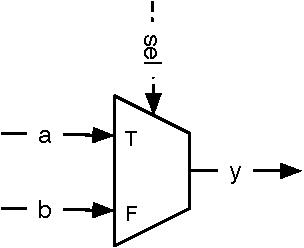
\includegraphics[scale=\scale]{../figures/mux}
\end{figure}
\shortlist{../code/mux.txt}
\begin{itemize}
\item So what?
\item Wait... What type is \code{a} and \code{b}?
\begin{itemize}
\item Can be any Chisel type!
\end{itemize}
\end{itemize}
\end{frame}

\begin{frame}[fragile]{Chisel has a Generic Multiplexer}
\begin{figure}
  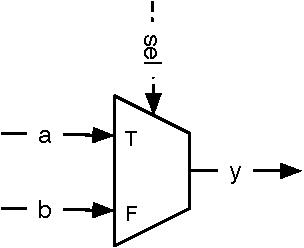
\includegraphics[scale=\scale]{../figures/mux}
\end{figure}
\shortlist{../code/mux.txt}
\begin{itemize}
\item SW people may not be impressed
\item They have generics since Java 1.5 in 2004
\begin{itemize}
\item \code{List<Flowers> != List<Cars>}
\end{itemize}
\end{itemize}
\end{frame}


\begin{frame}[fragile]{Generics in Hardware Construction}
\begin{itemize}
\item Chisel supports generic classes with type parameters
\item Write hardware generators independent of concrete type
\item This is a multiplexer \emph{generator}
\end{itemize}
\shortlist{../code/param_func.txt}
\end{frame}

\begin{frame}[fragile]{Put Generics Into Use}
\begin{itemize}
\item Let us implement a generic FIFO
\item Use the generic ready/valid interface from Chisel
\end{itemize}
\shortlist{../code/fifo_decoupled.txt}
\end{frame}

\begin{frame}[fragile]{Define the FIFO Interface}
\shortlist{../code/fifo_io.txt}
\begin{itemize}
\item We need enqueueing and dequeueing ports
\item Note the \code{Flipped}
\begin{itemize}
\item It switches the direction of ports
\item No more double definitions of an interface
\end{itemize}
\end{itemize}
\end{frame}

\begin{frame}[fragile]{But What FIFO Implementation?}
\begin{itemize}
\item Bubble FIFO (good for low data rate)
\item Double buffer FIFO (fast restart)
\item FIFO with memory and pointers (for larger buffers)
\begin{itemize}
\item Using flip-flops
\item Using on-chip memory
\end{itemize}
\item And some more...
\end{itemize}
\begin{itemize}
\item This calls for object-oriented \sout{programming} \emph{hardware construction}
\end{itemize}
\end{frame}

\begin{frame}[fragile]{Abstract Base Class and Concrete Extension}
\shortlist{../code/fifo_abstract.txt}
\begin{itemize}
\item May contain common code
\item Extend by concrete classes
\end{itemize}
\begin{chisel}
class BubbleFifo[T <: Data](gen: T, depth: Int) extends Fifo(gen: T, depth: Int) {
\end{chisel}
\end{frame}



\begin{frame}[fragile]{Select a Concrete FIFO Implementation}
\begin{itemize}
\item Decide at hardware generation
\item Can use all Scala/Java power for the decision
\begin{itemize}
\item Connect to a web service, get \sout{Google} Alphabet stock price, and decide on which to use ;-)
\item For sure a silly idea, but you see what is possible...
\item Developers may find clever use of the Scala/Java power
\item We could present a GUI to the user to select from
\end{itemize}
\item We use XML files parsed at hardware generation time
\item End of TCL, Python,... generated hardware
\end{itemize}
\end{frame}

\begin{frame}[fragile]{Binary to BCD Conversion for VHDL}
\begin{figure}
    \centering
    \includegraphics[scale=0.6]{JavaBCD}
\end{figure}
\end{frame}

\begin{frame}[fragile]{Java Program}
\begin{itemize}
\item Generates a VHDL table
\item The core code is:
\end{itemize}
\begin{chisel}
for (int i = 0; i < Math.pow(2, ADDRBITS); ++i) {
    int val = ((i/10)<<4) + i%10;
    // write out VHDL code for each line
\end{chisel}
\begin{itemize}
\item With all boilerplate 118 LoC
\end{itemize}
\end{frame}

\begin{frame}[fragile]{Chisel Version of Binary to BCD Conversion}
%\begin{chisel}
%  val array = new Array[Int](256)
%  for (i <- 0 to 99) {
%    array(i) = ((i/10)<<4) + i%10
%  }
%  val table = VecInit(array.map(_.U(8.W)))
%\end{chisel}
\begin{chisel}
  val table = Wire(Vec(100, UInt(8.W)))
  for (i <- 0 until 100) {
    table(i) := (((i/10)<<4) + i%10).U
  }
  val bcd = table(bin)
\end{chisel}
\begin{itemize}
\item Directly generates the hardware table as a \code{Vec}
\item At hardware construction time
\item In the same language
\end{itemize}
\end{frame}

\begin{frame}[fragile]{Use Functional Programming for Generators}
\shortlist{../code/fun_first.txt}
\shortlist{../code/fun_func_lit.txt}
\shortlist{../code/fun_reduce_tree.txt}
\begin{itemize}
\item This is a simple example
\item What about an arbiter tree with fair arbitration?
\end{itemize}
\end{frame}

\begin{frame}[fragile]{Functional Generation}
\begin{itemize}
\item Anonymous functions, called \emph{function literal}
\begin{chisel}
  (param) => function body
\end{chisel}
\item A function for a minimum search
\shortlist{../code/fun_min.txt}
\end{itemize}
\end{frame}

\begin{frame}[fragile]{Minimal Function with Index}
\begin{itemize}
\item Was the example for Tjark's heap sort
\shortlist{../code/fun_min2.txt}
\item We need an extra bundle to hold both values
\item A for loop is not so functional
\end{itemize}
\end{frame}

\begin{frame}[fragile]{We Can Use Tuples and zipWithIndex}
\begin{itemize}
\item \code{zipWithIndex} transforms the original sequence to a sequence of tuples
with second element is the index
\item Use \code{map} to translate from Scala \code{Int} to Chisel \code{UInt}
\item \code{reduce} does the minimum function, actually called 2 times (we could optimize this)
\shortlist{../code/fun_min3.txt}
\item The result is a Scala \code{Vector} and not a Chisel \code{Vec}
\end{itemize}
\end{frame}

\begin{frame}[fragile]{Solution with a Vec}
\begin{itemize}
\item Don't remember the details
\item But this results in a \code{Vec}
\shortlist{../code/fun_min4.txt}
\item
\item We should add a \code{reduceTree} to the Scala sequence version (\code{TraversableOnce})
\end{itemize}
\end{frame}

\begin{frame}[fragile]{An Arbiter}
\shortlist{../code/fun_arbiter.txt}
\end{frame}



\begin{frame}[fragile]{XXX}
\begin{itemize}
\item TODO: s4noc connection is part of the generator story
\item
\item
\end{itemize}
\end{frame}

\begin{frame}[fragile]{XXX}
\begin{itemize}
\item
\item
\item
\end{itemize}
\end{frame}



\begin{frame}[fragile]{Summary}
\begin{itemize}
\item Chisel is a library in Scala
\item RTL circuits are described in (plain) Chisel
\item Scala is the meta-circuit description language
\item Scala is used to write circuit generators
\item You write your tests in Scala
\end{itemize}
\end{frame}

\begin{frame}[fragile]{Simulation Lab Session}
\begin{itemize}
\item Components and Small Sequential Circuits
\item \url{https://github.com/schoeberl/chisel-lab/tree/master/lab3}
\end{itemize}
\end{frame}

\begin{frame}[fragile]{FPGA Lab Session}
\begin{itemize}
\item Examples from \url{https://github.com/schoeberl/chisel-examples}
\item Explore the ALU example
\begin{itemize}
\item It contains a tester
\item It can also be tested with the switches and LEDs on the FPGA
\end{itemize}
\item Explore the bubble FIFO example for wave form viewing
\item Do an example project from scratch
\begin{itemize}
\item But reuse Quartus files (from the ALU or knight example)
\item With a Chisel main
\item Some simple function with LEDs and switches
\begin{itemize}
\item E.g., moving light with direction change
\item Remember Knight Rider?
\end{itemize}
\item Running it in the FPGA
\end{itemize}
\end{itemize}
\end{frame}

\end{document}